%!TEX root = /Users/laura/Repositories/HandwritingRecognition/report/main.tex
% \resizebox {0.6\columnwidth} {!} {
	\begin{tikzpicture}
		[
			noname/.style={%
			rectangle,
			text height=1.5ex,
			text depth=.25ex,
			text width=1em,
			text centered,
			minimum height=1em
  		}]
	    \node[anchor=south west,inner sep=0] (image) at (0,0) {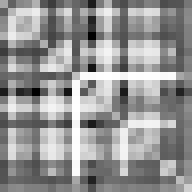
\includegraphics[width=0.65\columnwidth]{individual/img/discussion/distance.png}};
	    \def\keys{{"a", "b", "c", "d", "e", "f", "g", "h", "i", "k", "l", "m", "n", "o", "p", "q", "r", "s", "t", "u", "v", "x", "y", "z"}}
	    \begin{scope}[x={(image.south east)},y={(image.north west)}]
	    % 0.04166666667 = 1/24
	        \draw[help lines,xstep=.04166666667,ystep=.04166666667] (0,0) grid (1,1);
				\foreach \x in {0,1,...,23} { 
					\node [anchor=south, noname] at (\x/24 + 1/48, 1) {\small \pgfmathparse{\keys[\x]}\pgfmathresult}; 
				}
				\foreach \y in {0,1,...,23} { 
					\node [anchor=east, noname] at (0,1 - \y/24 - 1/48) {\small \pgfmathparse{\keys[\y]}\pgfmathresult}; 
				}
	    \end{scope}
	\end{tikzpicture}
% }